\documentclass{beamer}

\mode<presentation> {
  \usetheme{Singapore}
  \usefonttheme[onlymath]{serif}
}

% % % % to make navigation two lines
\usepackage{ragged2e}

\makeatletter
\setbeamertemplate{section in head/foot}{%
	\parbox[c][0.33cm][t]{\dimexpr(\textwidth-1.3cm)/\beamer@sectionmax\relax}{%
		\RaggedRight\fontsize{4}{4}\selectfont\insertsectionhead}}
\setbeamertemplate{footline}[frame number]
\makeatother
% % % %
\usepackage{booktabs, calc, rotating}
\usepackage{scalefnt}
\usepackage[english]{babel}
\usepackage[latin1]{inputenc}
\usepackage{times}
\usepackage{alltt}

  \setbeamertemplate{navigation symbols}{}
  \setbeamertemplate{blocks}[rounded][shadow=true]

%%%%%%%%%%%%%%%%%%%%%%%%%%%%%%%%%%%%%%%%%%%%%%%%%%%%%%%%%%%%%%%%%%%%%%%%%%%%%%%%%%%%
%  CHANGE THE TITLE AND INPUT FILE ACCORDING TO THE CHAPTER THAT YOU WISH TO COMPILE
%%%%%%%%%%%%%%%%%%%%%%%%%%%%%%%%%%%%%%%%%%%%%%%%%%%%%%%%%%%%%%%%%%%%%%%%%%%%%%%%%%%%

\title[Inference]{Statistical Inference}

\date[Fall 2016]{Fall 2016}
%Personal definitions - Bayes Regression
\def\bsb{\boldsymbol \beta}
\def\bsa{\boldsymbol \alpha}
\def\bsm{\boldsymbol \mu}
\def\bsS{\boldsymbol \Sigma}
\def\bsx{\boldsymbol \xi}

\begin{document}

\frame{\titlepage}

\begin{frame}
  \frametitle{Outline}
     \tableofcontents[part=1]
\end{frame}

\part<presentation>{Main Talk}


\section{Overview of Statistical Inference}

\begin{frame}[shrink=2]
\frametitle{Overview of Statistical Inference}
\begin{itemize}
\item A set of data (a \textbf{sample}) has been collected that is considered representative of a larger set (the \textbf{population}). This relationship is known as the \textbf{sampling frame}.
\item Often, we can describe the distribution of the population in terms of a limited (finite) number of terms called \textbf{parameters}. These are referred to as \textit{parametric distributions}. With \textbf{nonparametric} analysis, we do not limit ourselves to only a few parameters.
\item The \textbf{statistical inference} goal is to say something about the (larger) population based on the observed sample (we ``\emph{infer},'' not ``\emph{deduce}''). There are three types of statements:
 \begin{enumerate}
\item \textbf{Estimation}
\item \textbf{Hypothesis Testing}
\item \textbf{Prediction}
\end{enumerate}
\end{itemize}
\end{frame}

\begin{frame}[shrink=2]
\frametitle{Wisconsin Property Fund}
\begin{itemize}
\item Discuss ideas of statistical inference in the context of a sample from the Wisconsin Property Fund
\item Specifically, consider 1,377 \textit{individual} claims from 2010 experience (slightly different from the analysis of 403 average claims in Chapter 1)
\end{itemize}
\vspace{-.15in}
\begin{table}[htbp]\scalefont{0.7}
  \centering
    \begin{tabular}{l|rrrrrrr}
    \hline
                   &        &First     &       &         &Third        &        &Standard\\
                   & Minimum& Quartile &Median &Mean     & Quartile    &Maximum &Deviation \\  \hline
Claims             &1       & 788      &2,250  & 26,620  &  6,171      & 12,920,000 &368,030\\
Logarithmic Claims & 0      & 6.670    & 7.719 & 7.804   & 8.728       & 16.370 & 1.683\\
    \hline
    \end{tabular}
 \end{table}

\vspace{-.2in}
\begin{figure}[htp]
\begin{center}
    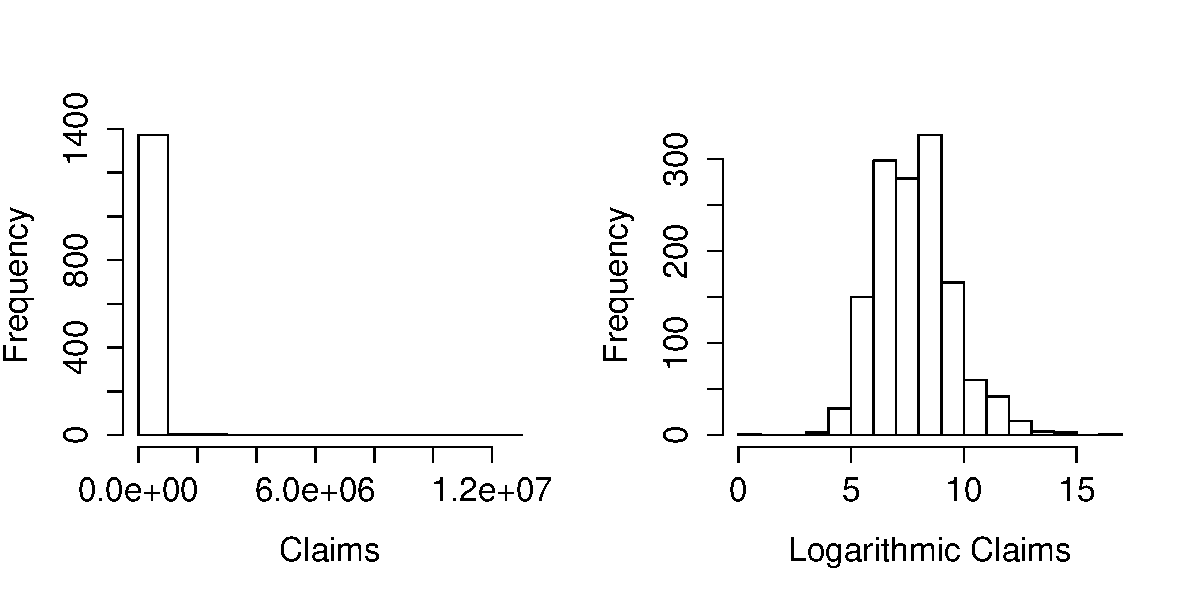
\includegraphics[width=.7\textwidth]{Figures/Severity2.pdf}
\end{center}
\end{figure}
\end{frame}

\begin{frame}[shrink=2]
\frametitle{Sampling Frame}
\begin{itemize}
\item In statistics, a sampling frame \textbf{error} occurs when the sampling frame, the list from which the
sample is drawn, is not an adequate approximation of the population of interest.
\item For the property fund example, the sample consists of all 2010 claims
\begin{itemize}\item The population might be all claims that could have potentially occurred in 2010.
\item Or, it might be all claims that could potentially occur, such as in 2010, 2011, and so forth\end{itemize}
\item A sample must be a representative subset of a  population, or ``universe,'' of interest. If the sample is not representative, taking a larger sample does not eliminate bias; you simply repeat the same mistake over again and again.
\end{itemize}
\end{frame}

\begin{frame}[shrink=2]
\frametitle{Sampling Frame II}
\begin{itemize}
\item A sample should be a representative subset of a population, or ``universe,'' of interest.
\item Formally
\begin{itemize}
\item We assume that the random variable $X$ represents a draw from a population with distribution function F(.)
\item We make several such draws ($n$), each unrelated to one another (statistically independent)
\item Sometimes we say that $X_1, \ldots, X_n$ is a random sample (with replacement) from F(.)
\item Sometimes we say that $X_1, \ldots, X_n$ are identically and independently distributed ($iid$)
\end{itemize}\end{itemize}
\end{frame}


\begin{frame}[shrink=2]
\frametitle{Describing the Population}
\begin{itemize}
\item We think of the random variable $X$ as a draw from the population with distribution function F(.)
\item There are several ways to summarize F(.). We might consider the mean, standard deviation, 95th percentile, and so on.
\begin{itemize}
\item Because these summary stats do not depend on a specific parametric reference, they are \textbf{nonparametric} summary measures.
\end{itemize}
\item In contrast, we can think of logarithmic claims as normally distributed with mean $\mu$ and standard deviation $\sigma$, that is, claims  have a \textit{lognormal} distribution
\item We will also look at the gamma distribution, with parameters $\alpha$ and $\theta$, as a claims model
\begin{itemize}
\item The normal, lognormal, and gamma are examples of \textbf{parametric} distributions.
\item The quantities $\mu$, $\sigma$, $\alpha$, and $\theta$ are known as \textit{parameters}. When we know the parameters of a distribution family, then we have knowledge of the entire distribution.
\end{itemize}
\end{itemize}
\end{frame}

\subsection{Estimation and Prediction}

\begin{frame}[shrink=2]
\frametitle{Estimation}
\begin{itemize}
\item Use $\theta$ to denote a summary of the population.
\begin{itemize}
\item Parametric - It can be a parameter from a distribution such as $\mu$ or $\sigma$.
\item Nonparametric - It can also be a nonparametric summary such as the mean or standard deviation.
\end{itemize}
\item Let $\hat{\theta} =\hat{\theta}(X_1, \ldots, X_n)$ be a function of the sample that provides proxy, or \textbf{estimate}, of $\theta$. It is a function of the sample $X_1, \ldots, X_n$.
\item In our property fund case,
\begin{itemize}
\item 7.804 is a (nonparametric) estimate of the population expected logarithmic claim and 1.683 is an estimate of the corresponding standard deviation.
\item These are (parametric) estimates of the normal distribution for logarithmic claims
\item The estimate of the expected claim using the lognormal distribution is 10,106.8 (=$\exp(7.804+1.683^2/2))$.
\end{itemize}
\end{itemize}
\end{frame}

\begin{frame}[shrink=2]
\frametitle{Lognormal Distribution and Estimation}
\begin{itemize}
\item Assume that claims follow a lognormal distribution, so that logarithmic claims follow the familiar normal distribution.
\item Specifically, assume $\ln X$ has a normal distribution with mean $\mu$ and variance $\sigma^2$, sometimes denoted as $X \sim N(\mu, \sigma^2)$.
\item For the property data, estimates are $\hat{\mu} =7.804$ and $\hat{\sigma} = 1.683$. The ``hat'' notation is common. These are said to be \textbf{point estimates}, a single approximation of the corresponding parameter.
\item Under general maximum likelihood theory (that we will do in a little bit), these estimates typically have a normal distribution for large samples.
\begin{itemize}
\item Using notation, $\hat{\theta}$ has an approximate normal distribution with mean $\theta$ and variance, say, $\mathrm{Var}(\hat{\theta})$.
\item Take the square root of the variance and plug-in the estimate to define $se(\hat{\theta}) = \sqrt{\mathrm{Var}(\hat{\theta})}$. A \textbf{standard error} is an estimated standard deviation.
\item The next step in the mathematical statistics theory is to establish that $ (\hat{\theta}-\theta)/se(\hat{\theta})$
has a $t$-distribution with ``degrees of freedom'' (a parameter of the distribution) equal to the sample size minus the dimension of  $\theta$.
\end{itemize}
\end{itemize}
\end{frame}

\begin{frame}[shrink=2]
\frametitle{Lognormal Distribution and Estimation II}
\begin{itemize}
\item Assume that claims follow a lognormal distribution, so that logarithmic claims follow the familiar normal distribution.
\item Under general maximum likelihood theory
\begin{itemize}
\item $\hat{\theta}$ has an approximate normal distribution with mean $\theta$ and variance, say, $\mathrm{Var}(\hat{\theta})$.
\item Take the square root of the variance and plug-in the estimate to define $se(\hat{\theta}) = \sqrt{\mathrm{Var}(\hat{\theta})}$. A \textbf{standard error} is an estimated standard deviation.
\item $ (\hat{\theta}-\theta)/se(\hat{\theta})$
has a $t$-distribution with ``degrees of freedom'' (a parameter of the distribution) equal to the sample size minus the dimension of  $\theta$.
\item As an application, we can invert this result to get a \textbf{confidence interval} for $\theta$.
\end{itemize}
\item A pair of statistics, $\hat{\theta}_1$ and $\hat{\theta}_2$, provide an interval of the form $[\hat{\theta}_1, \hat{\theta}_2]$ This interval is a $1-\alpha$ confidence interval for $\theta$ if $\Pr\left(\hat{\theta}_1 \le \theta \le \hat{\theta}_2\right) \ge 1-\alpha.$
\item For example, $\hat{\theta}_1 = \hat{\mu} - (t-value) \hat{\sigma}/\sqrt{n}$ and $\hat{\theta}_2 = \hat{\mu} + (t-value) \hat{\sigma}/\sqrt{n}$ provide a confidence interval for $\theta=\mu$. When $\alpha = 0.05$, $t-value \approx 1.96$.
\item For the property fund, (7.715235, 7.893208) is a 95\% confidence interval for $\mu$.
\end{itemize}
\end{frame}

\begin{frame}[shrink=2]
\frametitle{Lognormal Distribution and Hypothesis Testing}
An important statistical inference procedure involves verifying ideas about parameters.
\begin{itemize}
\item To illustrate, in the property fund, assume that mean logarithmic claims have historically been approximately been $\mu_0 = log(5000)= 8.517$. I might want to use 2010 data to see whether the mean of the distribution has changed. I also might want to test whether it has increased.
\item The actual 2010 average was $\hat{\mu} =7.804$. Is this a significant departure from $\mu_0 = 8.517$?
\item One way to think about it is in terms of standard errors. The deviation is $(8.517-7.804)/(1.683/\sqrt{1377}) = 15.72$ standard errors. This is highly unlikely assuming an approximate normal distribution.
\end{itemize}
\end{frame}

\begin{frame}[shrink=2]
\frametitle{Lognormal Distribution and Hypothesis Testing II}
\begin{itemize}
\item One hypothesis testing procedure begin with the calculation the test statistic $ t-stat=(\hat{\theta}-\theta_0)/se(\hat{\theta})$. Here, $\theta_0$ is an assumed value of the parameter.
\item Then, one rejects the hypothesized value if the test statistic $t-stat$ is ``unusual.'' To gauge ``unusual,'' use the same $t$-distribution as introduced for confidence intervals.
\item If you only want to know about a difference, this is known as a ``two-sided'' test; use the same $t-value$ as the case for confidence intervals.
\item If you want to investigate whether there has been an increase (or decrease), then use a ``one-sided'' test.
\item Another useful concept in hypothesis testing is the $p$-value, which is short hand for probability value. For a data set, a $p$-value is defined to be the smallest significance level for which the null hypothesis would be rejected.
\end{itemize}
\end{frame}

\begin{frame}[shrink=2]
\frametitle{Property Fund -- Other Distributions}
\scalefont{0.9}
\begin{itemize}
\item For numerical stability and extensions to regression applications, statistical packages often work with transformed version of parameters
\item The following estimates are from the \textbf{R} package \textbf{VGAM} (the {\tt{vglm}} function)
\end{itemize}
\begin{center}
\scalefont{0.9}
\begin{tabular}{l|rrr}\hline
Distribution &    Parameter & Standard & $t$-stat  \\
            & Estimate & Error & \\\hline
Gamma       &     10.190 &      0.050 &    203.831 \\
            &     -1.236 &      0.030 &    -41.180 \\
Lognormal   &      7.804 &      0.045 &    172.089 \\
            &      0.520 &      0.019 &     27.303 \\
Pareto     &      7.733 &      0.093 &     82.853 \\
           &     -0.001 &      0.054 &     -0.016 \\
GB2        &      2.831 &      1.000 &      2.832 \\
           &      1.203 &      0.292 &      4.120 \\
           &      6.329 &      0.390 &     16.220 \\
           &      1.295 &      0.219 &      5.910 \\\hline
\end{tabular}
\end{center}
\end{frame}



\section{Maximum Likelihood Theory}

\begin{frame}[shrink=2]
\frametitle{Likelihood Function}
\begin{itemize}
\item Let $\mathrm{f}(\cdot;\boldsymbol\theta)$ be the probability mass function if $X$ is discrete or the probability density function if it is continuous.
\item The likelihood is a function of the parameters ($\boldsymbol \theta$) with the data ($\mathbf{x}$)  fixed rather than a function of the data with the parameters fixed.
\item Define the \emph{log-likelihood function},
\begin{equation*}
L(\boldsymbol \theta) = L(\mathbf{x};\boldsymbol \theta ) = \ln \mathrm{f}(\mathbf{x};\boldsymbol \theta) = \sum_{i=1}^n \ln \mathrm{f}(x_i;\boldsymbol \theta),
\end{equation*}
evaluated at a realization $\mathbf{x}$.
\item In the case of independence, the joint density function can be expressed as a product of the marginal
density functions and, by taking logarithms, we can work with sums.

\end{itemize}
\end{frame}

\begin{frame}[shrink=2]
\frametitle{Example. Pareto Distribution}
\begin{itemize}
\item Suppose that $X_1, \ldots, X_n$ represent a random sample from a single-parameter Pareto with cumulative distribution function:
\begin{equation*}
\mathrm{F}(x) = 1- \left(\frac{500}{x}\right)^{\alpha}, ~~~~ x>500 .
\end{equation*}
\item In this case, the single parameter is $\theta = \alpha$.
\item The corresponding probability density function is $\mathrm{f}(x) = 500^{\alpha} \alpha x^{-\alpha-1}$
and the logarithmic likelihood is
\begin{equation*}
L(\boldsymbol \alpha) = \sum_{i=1}^n \ln \mathrm{f}(x_i;\alpha) = n \alpha \ln 500 +n \ln \alpha -(\alpha+1)  \sum_{i=1}^n \ln x_i .
\end{equation*}
\end{itemize}
\end{frame}

\begin{frame}[shrink=2]
\frametitle{Properties of Likelihood Functions}
\begin{itemize}
\item One basic property of likelihood functions is:
\begin{equation*}\label{E11:ScoreZero}
\mathrm{E} \left( \frac{ \partial}{\partial \boldsymbol \theta}
L(\boldsymbol \theta) \right) = \mathbf 0
\end{equation*}
\item The derivative of the log-likelihood function, $\partial L(\boldsymbol \theta)/\partial \boldsymbol \theta$, is called the
\emph{score function}.
\item To see this,
\begin{eqnarray*}
\mathrm{E} \left( \frac{ \partial}{\partial \boldsymbol \theta} L(\boldsymbol \theta) \right)
&=& \mathrm{E} \left( \frac{\frac{\partial}{\partial \boldsymbol \theta}\mathrm{f}(\mathbf{x};\boldsymbol \theta)}{\mathrm{f}(\mathbf{x};\boldsymbol \theta )}  \right)
= \int\frac{\partial}{\partial \boldsymbol \theta} \mathrm{f}(\mathbf{x};\boldsymbol \theta ) d \mathbf y \\
&=& \frac{\partial}{\partial \boldsymbol \theta} \int \mathrm{f}(\mathbf{x};\boldsymbol \theta ) d \mathbf y
= \frac{\partial}{\partial \boldsymbol \theta} 1 = \mathbf 0.
\end{eqnarray*}
\end{itemize}
\end{frame}

\begin{frame}[shrink=2]
\frametitle{Properties of Likelihood Functions II}
\begin{itemize}
\item Another basic property is:
\begin{equation*}\label{E11:HessianZero}
\mathrm{E} \left( \frac{ \partial^2}{\partial \boldsymbol \theta
\partial \boldsymbol \theta^{\prime}} L(\boldsymbol \theta) \right)
+ \mathrm{E} \left( \frac{ \partial L(\boldsymbol \theta)}{\partial
\boldsymbol \theta} \frac{ \partial L(\boldsymbol \theta)}{\partial
\boldsymbol \theta^{\prime}}
 \right) = \mathbf 0.
\end{equation*}
\item With this, we can define the \emph{information matrix}
\begin{equation*}\label{E11:InfoMatrix}
\mathbf{I}(\boldsymbol \theta) = \mathrm{E} \left( \frac{ \partial
L(\boldsymbol \theta)}{\partial \boldsymbol \theta} \frac{ \partial
L(\boldsymbol \theta)}{\partial \boldsymbol \theta^{\prime}}
 \right) = -\mathrm{E} \left( \frac{ \partial^2}{\partial \boldsymbol \theta
\partial \boldsymbol \theta^{\prime}} L(\boldsymbol \theta) \right).
\end{equation*}
\item In general
\begin{equation*}
\frac{ \partial}{\partial \boldsymbol \theta} L(\boldsymbol \theta)
=\frac{ \partial}{\partial \boldsymbol \theta} \ln \prod_{i=1}^n
\mathrm{f}(x_i;\boldsymbol \theta ) =\sum_{i=1}^n \frac{
\partial}{\partial \boldsymbol \theta}
\ln \mathrm{f}(x_i;\boldsymbol \theta ).
\end{equation*}
has a large sample \textbf{normal distribution} with mean \textbf{0} and variance $\mathbf{I}(\boldsymbol \theta)$.
\end{itemize}
\end{frame}

\begin{frame}[shrink=2]
\frametitle{Maximum Likelihood Estimators}
\begin{itemize}
\item The value of $\boldsymbol \theta$, say $\boldsymbol \theta_{MLE}$, that maximizes $\mathrm{f}(\mathbf{x};\boldsymbol \theta)$ is called the\emph{ maximum likelihood estimator}.
\item Maximum likelihood estimators are values of the parameters $\boldsymbol \theta$ that are ``most likely'' to have been produced by the data.
\item Because $\ln(\cdot)$ is a one-to-one function, we can also determine $\boldsymbol \theta_{MLE}$ by maximizing the log-likelihood function, $L(\boldsymbol \theta)$.
\end{itemize}

\bigskip

\noindent\textbf{Example. Course C/Exam 4. May 2000, 21.} You are given the following five observations: 521, 658, 702, 819, 1217. You use the single-parameter Pareto with cumulative distribution function:
\begin{equation*}
\mathrm{F}(x) = 1- \left(\frac{500}{x}\right)^{\alpha}, ~~~~ x>500 .
\end{equation*}
Calculate the maximum likelihood estimate of the parameter $\alpha$.
\end{frame}

\begin{frame}[shrink=2]
\frametitle{Instructor Notes}
\noindent\textbf{Example. Course C/Exam 4. May 2000, 21.} You are given the following five observations: 521, 658, 702, 819, 1217. You use the single-parameter Pareto with cumulative distribution function:
\begin{equation*}
\mathrm{F}(x) = 1- \left(\frac{500}{x}\right)^{\alpha}, ~~~~ x>500 .
\end{equation*}
Calculate the maximum likelihood estimate of the parameter $\alpha$.

\bigskip

\textit{Solution}. With $n=5$, the logarithmic likelihood is
\begin{equation*}
L(\alpha ) =  \sum_{i=1}^5 \ln \mathrm{f}(x_i;\alpha ) =  5 \alpha \ln 500 + 5 \ln \alpha
-(\alpha+1) \sum_{i=1}^5 \ln x_i.
\end{equation*}
Solving for the root of the score function yields
\begin{equation*}
\frac{ \partial}{\partial \alpha } L(\alpha ) =    5  \ln 500 + 5 / \alpha -  \sum_{i=1}^5 \ln x_i
=_{set} 0 \Rightarrow \alpha_{MLE} = \frac{5}{\sum_{i=1}^5 \ln x_i - 5  \ln 500 } = 2.453 .
\end{equation*}
\end{frame}

\begin{frame}[shrink=2]
\frametitle{Asymptotic Normality of Maximum Likelihood Estimators}
\begin{itemize}
\item Under broad conditions, $\boldsymbol \theta_{MLE}$ has a large sample normal distribution with mean $\boldsymbol \theta$ and variance $\left( \mathbf{I}(\boldsymbol \theta) \right)^{-1}$.
\item  $2 \left( L(\boldsymbol \theta_{MLE}) - L(\boldsymbol \theta) \right)$  has a chi-square distribution with degrees of freedom equal to the dimension of $\boldsymbol \theta$ .
\item These are critical results upon which much of estimation and hypothesis testing is based.
\bigskip

\noindent\textbf{Example. Course C/Exam 4. Nov 2000, 13.} A sample of ten observations comes from a parametric family $f(x,; \theta_1, \theta_2)$ with log-likelihood function
\begin{equation*}
L(\theta_1, \theta_2)= \sum_{i=1}^{10} f(x_i; \theta_1, \theta_2) = -2.5 \theta_1^2 - 3
\theta_1 \theta_2 - \theta_2^2 + 5 \theta_1 + 2 \theta_2 + k,
\end{equation*}
where $k$ is a constant. Determine the estimated covariance matrix of the maximum likelihood estimator, $\hat{\theta_1}, \hat{\theta_2} $.
\end{itemize}
\end{frame}


\begin{frame}[shrink=2]
\frametitle{Instructor Notes}
\noindent\textbf{Example. Course C/Exam 4. Nov 2000, 13.} A sample of ten observations comes from a
parametric family $f(x,; \theta_1, \theta_2)$ with log-likelihood function
\begin{equation*}
L(\theta_1, \theta_2)= \sum_{i=1}^{10} f(x_i; \theta_1, \theta_2) = -2.5 \theta_1^2 - 3
\theta_1 \theta_2 - \theta_2^2 + 5 \theta_1 + 2 \theta_2 + k,
\end{equation*}
where $k$ is a constant. Determine the estimated covariance matrix of the maximum likelihood
estimator, $\hat{\theta_1}, \hat{\theta_2} $.

\textit{Solution}. The matrix of second derivatives is
\begin{equation*}
\left(
\begin{array}{cc}
  \frac{ \partial ^2}{\partial \theta_1 ^2 } L & \frac{ \partial ^2}{\partial \theta_1 \partial \theta_2 } L  \\
  \frac{ \partial ^2}{\partial \theta_1 \partial \theta_2 } L & \frac{ \partial ^2}{\partial \theta_1 ^2 } L
\end{array} \right) =
\left(
\begin{array}{cc}
  -5 & -3  \\
  -3 & -2
\end{array} \right)
\end{equation*}
Thus, the information matrix is:
\begin{equation*}
\mathbf{I}(\theta_1, \theta_2) = -\mathrm{E} \left( \frac{ \partial^2}{\partial \boldsymbol \theta
\partial \boldsymbol \theta^{\prime}} L(\boldsymbol \theta) \right) = \left(
\begin{array}{cc}
  5 & 3  \\
  3 & 2
\end{array} \right)
\end{equation*}
and
\begin{equation*}
\mathbf{I}^{-1}(\theta_1, \theta_2) = \frac{1}{5(2) - 3(3)}\left(
\begin{array}{cc}
  2 & -3  \\
  -3 & 5
\end{array} \right) = \left(
\begin{array}{cc}
  2 & -3  \\
  -3 & 5
\end{array} \right) .
\end{equation*}
\end{frame}

\begin{frame}[shrink=2]
\frametitle{Maximum Likelihood Estimation (MLE)}
\begin{itemize}
\item Why use maximum likelihood estimation?
\begin{itemize}
\item General purpose tool - works in many situations (data can be censored, truncated, include covariates, time-dependent, and so forth)
\item It is ``optimal,'' the best, in the sense that it has the smallest variance among the class of all unbiased estimators. (Caveat: for large sample sizes).
\end{itemize}
\item A drawback: Generally, maximum likelihood estimators are computed iteratively, no closed-form solution.
\begin{itemize}
\item For example, you may recall a ``Newton-Raphson'' iterative algorithm from calculus
\item Iterative algorithms require starting values. For some problems, the choice of a close starting value is critical.
\end{itemize}
\end{itemize}
\end{frame}

\begin{frame}[shrink=2]
\frametitle{MLE and Statistical Significance}
One important type inference is to say whether a parameter estimate is ``statistically significant''
\begin{itemize}
\item We learned earlier that $\boldsymbol \theta_{MLE}$ has a large sample normal distribution with mean $\boldsymbol \theta$ and variance $\left( \mathbf{I}(\boldsymbol \theta) \right)^{-1}$.
\item Look to the $j$th element of $\boldsymbol \theta_{MLE}$, say $\theta_{MLE,j}$.
\item Define $se(\theta_{MLE,j})$, the standard error (estimated standard deviation) to be square root of the $j$ diagonal element of $\left( \mathbf{I}(\boldsymbol \theta)_{MLE} \right)^{-1}$.
\item To assess the hypothesis that $\theta_j$ is 0, we look at the rescaled estimate $t(\theta_{MLE,j})=\theta_{MLE,j}/se(\theta_{MLE,j})$. It is said to be a $t$-statistic or $t$-ratio.
\item Under this hypothesis, it has a $t$-distribution with degrees of freedom equal to the sample size minus the dimension of $\boldsymbol \theta_{MLE}$.
\item For most actuarial applications, the $t$-distribution is very close to the (standard) normal distribution. Thus, sometimes this ratio is also known a $z$-statistic or ``$z$-score.''
\end{itemize}
\end{frame}

\begin{frame}[shrink=2]
\frametitle{MLE and Statistical Significance II}
Assessing Statistical Significance
\begin{itemize}
\item If the $t$-statistic $t(\theta_{MLE,j})$ exceeds a cut-off (in absolute value), then the $j$th variable is said to be ``statistically significant.''
\begin{itemize}
\item For example, if we use a 5\% significance level, then the cut-off is 1.96 using a normal distribution approximation.
\item More generally, using a $100 \alpha \%$ significance level, then the cut-off is a  $100(1-\alpha/2)\%$ quantile from a $t$-distribution using degrees of freedom equal to the sample size minus the dimension of $\boldsymbol \theta_{MLE}$.
\end{itemize}
\item Another useful concept in hypothesis testing is the $p$-value, shorthand for probability value.
\begin{itemize}
\item For a data set, a $p$-value is defined as the smallest significance level for which the null hypothesis would be rejected.
\item The $p$-value is a useful summary statistic for the data analyst to report because it allows the reader to understand the strength of the deviation from the null hypothesis.
\end{itemize}
\end{itemize}
\end{frame}


\begin{frame}[shrink=2]
\frametitle{MLE and Model Validation}
Another important type inference is to select a model from two choices, where one choice is a subset of the other
\begin{itemize}
\item Suppose that we have a (large) model and determine the maximum likelihood estimator, $\boldsymbol \theta_{MLE}$.
\item Now assume that $p$ elements in $\boldsymbol \theta$ are equal to zero and determine the maximum likelihood estimator over the remaining set. Call this estimator  $\boldsymbol \theta_{Reduced}$
\item The statistic, $LRT= 2 \left( L(\boldsymbol \theta_{MLE}) - L(\boldsymbol \theta_{Reduced}) \right)$, is called the likelihood ratio (a difference of the logs is the log of the ratio. Hence, the term ``ratio.'')
\item Under the hypothesis that the reduce model is correct, the likelihood ratio has a chi-square distribution with degrees of freedom equal to $p$, the number of variables set equal to zero.
\item This allows us to judge which of the two models is correct. If the statistic $LRT$ is large relative to the chi-square distribution, then we reject the simpler, reduced, model in favor of the larger one.
\end{itemize}
\end{frame}

\begin{frame}[shrink=2]
\frametitle{Information Criteria}
\begin{itemize}
\item These statistics can be used when comparing several alternative models that are not necessarily nested. One picks the model that minimizes the criterion.
\item \emph{Akaike's Information Criterion}
\begin{equation*}
AIC = -2 \times L(\boldsymbol \theta_{MLE}) + 2 \times (number~of~parameters)
\end{equation*}
\begin{itemize}\item The additional term $2 \times $ $(number~of~parameters)$ is a penalty for the complexity of the model.
\item Other things equal, a more complex model means more parameters, resulting in a larger value of the criterion.
\end{itemize}
\item \emph{Bayesian Information Criterion}, defined as
\begin{equation*}
BIC = -2 \times L(\boldsymbol \theta_{MLE}) + (number~of~parameters) \times \ln (number~of~observations)
\end{equation*}
\begin{itemize}\item This measure gives greater weight to the number of parameters.
\item Other things being equal, $BIC$ will suggest a more parsimonious model than $AIC$.
\end{itemize}
\end{itemize}
\end{frame}

\begin{frame}[shrink=2]
\frametitle{Property Fund Information Criteria}
\begin{itemize}
\item Both the $AIC$ and $BIC$ statistics suggest that the \textit{GB2} is the best fitting model whereas gamma is the worst.
\end{itemize}
\begin{center}
\scalefont{0.9}
\begin{tabular}{l|rr} \hline
Distribution &        AIC &        BIC \\ \hline
     Gamma &   28,305.2 &   28,315.6 \\
 Lognormal &   26,837.7 &   26,848.2 \\
    Pareto &   26,813.3 &   26,823.7 \\
       GB2 &   26,768.1 &   26,789.0 \\ \hline
\end{tabular}\end{center}
\end{frame}



\begin{frame}[shrink=2]
\frametitle{Property Fund Fitted Distributions}
\begin{itemize}
\item In this graph, black represents actual (smoothed) logarithmic claims
\item Best approximated by green which is fitted GB2
\item Pareto (purple) and Lognormal (lightblue) are also pretty good
\item Worst are the exponential (in red) and gamma (in dark blue)
\end{itemize}

\vspace{-.2in}
\begin{figure}[htp]
\begin{center}
    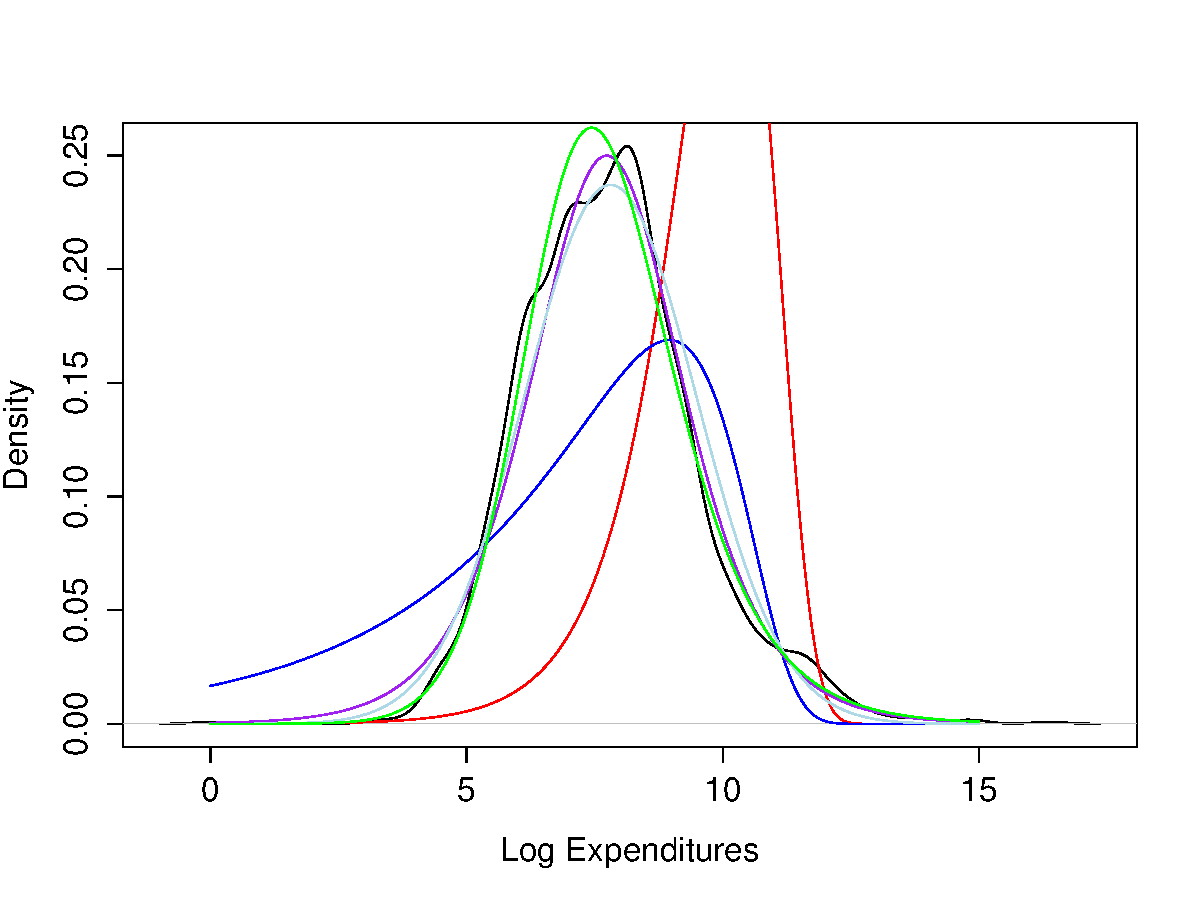
\includegraphics[width=.8\textwidth]{Figures/PropertyFundFittedSeverities.pdf}
\end{center}
\end{figure}
\end{frame}


\end{document}

\begin{frame}[shrink=2]
\frametitle{Instructor Notes}
\begin{itemize}
\item
\end{itemize}
\end{frame}



\textcolor{blue}{temp}

